%\title{LaTeX Portrait Poster Template}
%%%%%%%%%%%%%%%%%%%%%%%%%%%%%%%%%%%%%%%%%
% a0poster Portrait Poster
% LaTeX Template
% Version 1.0 (22/06/13)
%
% The a0poster class was created by:
% Gerlinde Kettl and Matthias Weiser (tex@kettl.de)
% 
% Adapter by Jens Buysse for Hogeschool Gent
% This template has been downloaded from:
% http://www.LaTeXTemplates.com
%
% License:
% CC BY-NC-SA 3.0 (http://creativecommons.org/licenses/by-nc-sa/3.0/)
%
%%%%%%%%%%%%%%%%%%%%%%%%%%%%%%%%%%%%%%%%%

%----------------------------------------------------------------------------------------
%	PACKAGES AND OTHER DOCUMENT CONFIGURATIONS
%----------------------------------------------------------------------------------------

\documentclass[a0,portrait]{a0poster}

\usepackage{multicol} % This is so we can have multiple columns of text side-by-side
\columnsep=100pt % This is the amount of white space between the columns in the poster
\columnseprule=3pt % This is the thickness of the black line between the columns in the poster

\usepackage[svgnames]{xcolor} % Specify colors by their 'svgnames', for a full list of all colors available see here: http://www.latextemplates.com/svgnames-colors

\usepackage{times} % Use the times font
%\usepackage{palatino} % Uncomment to use the Palatino font

\usepackage{graphicx} % Required for including images
\graphicspath{{figures/}} % Location of the graphics files
\usepackage{booktabs} % Top and bottom rules for table
\usepackage[font=small,labelfont=bf]{caption} % Required for specifying captions to tables and figures
\usepackage{amsfonts, amsmath, amsthm, amssymb} % For math fonts, symbols and environments
\usepackage{wrapfig} % Allows wrapping text around tables and figures
\usepackage[export]{adjustbox}

\begin{document}

%----------------------------------------------------------------------------------------
%	POSTER HEADER 
%----------------------------------------------------------------------------------------

% The header is divided into two boxes:
% The first is 75% wide and houses the title, subtitle, names, university/organization and contact information
% The second is 25% wide and houses a logo for your university/organization or a photo of you
% The widths of these boxes can be easily edited to accommodate your content as you see fit

\begin{minipage}[t]{0.75\linewidth}
\VeryHuge \color{HoGentAccent1} \textbf{Integratie van Machine Learning aan taxonomie-systeem van PIMLayer.} \color{Black}\\ % Title
\Huge\textit{Een vergelijkende studie tussen \newline verschillende aanbieders van Machine Learning as a Service}\\[2.4cm] % Subtitle
\huge \textbf{Jules Vervaeke, Pascal Synaeve, Koen Mertens}\\[0.5cm] % Author(s)
\huge Hogeschool Gent, Valentin Vaerwyckweg 1, 9000 Gent\\[0.4cm] % University/organization
\Large \texttt{jules.vervaeke@student.hogent.be} \\
\end{minipage}
%
\begin{minipage}[t]{0.25\linewidth}
\includegraphics[width=13cm,right]{figures/HOGENT_Logo_Pos_rgb.png} 

\end{minipage}

\vspace{1cm} % A bit of extra whitespace between the header and poster content

%----------------------------------------------------------------------------------------

\begin{multicols}{2} % This is how many columns your poster will be broken into, a portrait poster is generally split into 2 columns

%----------------------------------------------------------------------------------------
%	ABSTRACT
%----------------------------------------------------------------------------------------

\color{HoGentAccent1} % Navy color for the abstract

\begin{abstract}
Product Information Management (PIM) systemen bundelen informatie uit verschil- lende bronnen en creëren zo een single source of truth. PIMLayer is een bedrijf dat PIM systemen aanbiedt die nog door hun klanten kunnen worden geconfigureerd. Deze PIM systemen werken met een taxonomie systeem dat de gebruikers toe- laat om complexe query’s op een intuïtieve en efficiënte manier op te stellen en uit te voeren. Tot op heden moeten de tags uit de taxonomie systemen door de gebruikers met de hand worden toegevoegd aan de entiteiten, wat voor een grote werklast zorgt bij de klanten van PIMLayer. Om deze werklast te verlichten zou er gebruik kunnen gemaakt worden van machine learning modellen die de tags van de entiteiten in het systeem kunnen voorspellen. Deze modellen kunnen worden getraind en gedeployed door gebruik te maken van Machine Learning as a Service (MLaaS) providers. In deze bachelorproef wordt er onderzocht welke provider van MLaaS het best past bij deze specifieke use case. Hierbij kan er worden gekeken naar welke provider best presteert bij kleinere datasets, de prijs en gebruiksvrien- delijkheid. In deze studie worden 3 verschillende providers van MLaaS vergeleken: AWS SageMaker, Azure Machine Learning Services en Google Cloud Platform.
Om de prestaties van deze providers te vergelijken wordt er gebruik gemaakt van een dataset afkomstig van een PIM systeem dat reeds bestaat en van tags is voor- zien. Uit deze dataset worden er 5 datasets gemaakt: 1 met een grootte van 10, 20, 30, 50 en 100\% van de originele dataset. Door gebruik te maken van deze 5 data- sets, kunnen we de nauwkeurigheden en de gewogen nauwkeurigheden van de modellen die de providefrs genereerden vergelijken. Het minimum aantal records in de trainingsdataset bij Google Cloud Platform is 1000, wat deze provider een on- geschikt maakt voor deze use case. Azure kon voor elke dataset een betere nauw- keurigheid en gewogen nauwkeurigheid voorleggen en kan goedkoper worden geconfigureerd dan AWS SageMaker. Daardoor is Azure Machine Learning Servi- ces de beste optie om effectief te integreren in de PIM systemen van PIMLayer.
\end{abstract}
%----------------------------------------------------------------------------------------
%	INTRODUCTION
%----------------------------------------------------------------------------------------

\color{HoGentAccent1} 
\section*{Introductie}
\color{black}
\color{black}
Product Information Management (PIM)-systemen zijn alomtegenwoordig in de huidige e-commerce wereld, ze bundelen informatie uit verschillende bronnen om een single source of truth te creëren. PIMLayer is een Gents bedrijf dat PIM-systemen aanbiedt. Het biedt een standaard oplossing aan die bedrijven zelf kunnen aanpas- sen naar hun eigen noden en wensen. Het mikt vooral op kleine Vlaamse KMO’s die nog geen PIM-systeem hebben. PIMLayer werkt met een taxonomie systeem waardoor er zeer performante en precieze query’s kunnen worden opgesteld door de gebruiker.

Het taxonomie systeem dat PIMLayer gebruikt is een zeer grote troef ten opzichte van andere aanbieders van PIM-systemen, maar het zorgt ook voor een uitdaging: alle labels moeten door de gebruiker zelf worden toegevoegd. Dit zorgt voor een grote work-load bij de klant zelf. Zoals eerder al vermeld, bestaat het cliënteel van PIMLayer vooral uit kleinere Vlaamse KMO’s, die vaak weinig tot geen tijd hebben om zich bezig te houden met die taak. De oplossing voor dit probleem zou een slimme onboarding-tool kunnen zijn die, gebruikmakend van machine learning, slimme suggesties kan doen naar de klant toe en eventueel zelfstandig labels kan toevoegen aan het systeem.
%----------------------------------------------------------------------------------------
%	GEOLOGY
%----------------------------------------------------------------------------------------

\color{Black} % DarkSlateGray color for the rest of the content
\color{HoGentAccent1} 
\section*{Experimenten}
\color{black}
Om de verschillende providers van Machine Learning as a service te vergelijken, werd de data uit een bestaan PIM systeem gebruikt om modellen te trainen en testen. De originele dataset (kleine 1000 pdf-files) werd gebruikt om 5 datasets op te bouwen, 1 met 10\%, 20\%, 30\%, 50\% en 100\% van de originele dataset. Door deze 5 verschillende datasets te gebruiken kon er ook meer inzicht worden verworven over de leercurves van de modellen in functie van de grote van de dataset. Wat wel vrij relevant is voor de use-case van PIMLayer aangezien er zo snel mogelijk wil worden gestart met het geven van slimme suggesties en het autonoom laten taggen door het systeem.  

\color{HoGentAccent1} 
\section*{Resultaten}
\color{black}
Het is duidelijk dat Azure betere resultaten kan voorleggen voor deze use-case dan AWS, zowel de nauwkeurigheid \ref{nauwkeurigheid_chart} als de gewogen nauwkeurigheid \ref{gewogen_nauwkeurigheid_chart} zijn voor alle data-sets hoger.  
\begin{center}\vspace{1cm}
    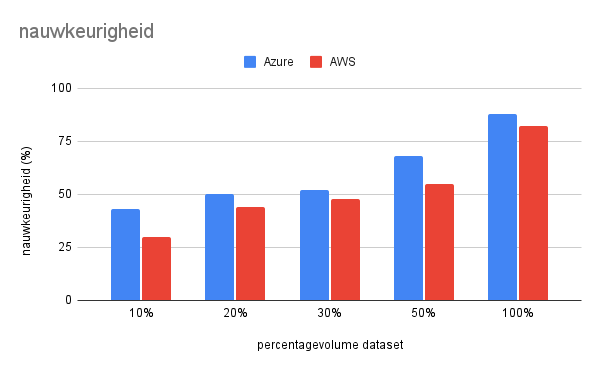
\includegraphics[width=1.0\linewidth]{nauwkeurigheid}
    \captionof{figure}{\color{HoGentAccent5} Bar chart die de nauwkeurigheden van AWS en Azure vergelijkt per percentage van de dataset dat werd gebruikt als trainingsdata.}
\end{center}\vspace{1cm}

\begin{center}\vspace{1cm}
    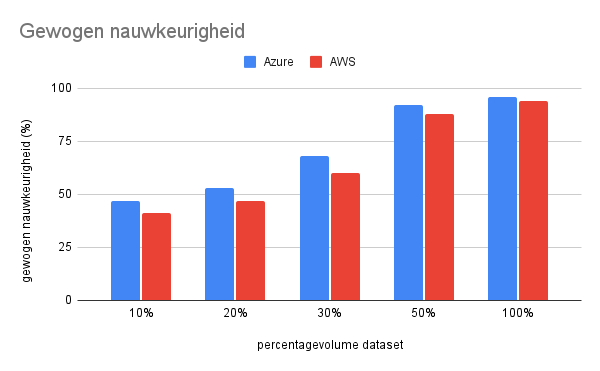
\includegraphics[width=1.0\linewidth]{Gewogen nauwkeurigheid}
    \captionof{figure}{\color{HoGentAccent5}Bar chart die de gewogen nauwkeurigheden van AWS en Azure vergelijkt per percentage van de dataset dat werd gebruikt als trainingsdata.}
\end{center}\vspace{1cm}
De gewogen nauwkeurigheid bereikt reeds 92\% wanneer 50\% van de originele dataset wordt gebruikt als trainingsdataset. 
\color{HoGentAccent1} 
\section*{Beslissen}
\color{HoGentAccent1} 
\subsection*{Proof of Concept}
\color{black}
De eerste vraag die moet worden gesteld is of de modellen die zijn gegenereerd überhaupt zouden kunnen helpen bij het on-boarding proces van een nieuw PIM-systeem. Het is duidelijk dat voor beide providers de modellen die gegeneerd werden op basis van de datasets die respectievelijk 10\%, 20\% en 30\% van de originele dataset bevatten, zeker niet geschikt zijn voor het autonoom toevoegen van tags aan de entiteiten van het systeem. Zowel het model van Azure als het model van AWS die met 50\% (350 records) van de originele dataset werden gegenereerd zijn zeker geschikt voor het geven van gerichte suggesties, en eventueel ook al voor het zelfstandig taggen van entiteiten. Beide modellen die werden gegenereerd met de originele dataset zijn zeker geschikt voor het geven van suggesties en ook voor het zelfstandig taggen. Dit wil zeggen dat het integreren van Machine Learning in het taxonomie systeem van PIMLayer zou kunnen helpen bij zowel het onboarding proces als bij het onderhouden en updaten van een bestaand PIM-systeem. Dat laatste is ook interessant voor andere PIM-systemen, zoals het systeem waar de Constructalia-dataset werd uit gehaald. 
\color{HoGentAccent1} 
\subsection*{AWS of Azure}
\color{black}
Voorlopig gebruikt PIMLayer geen specifieke AWS of Azure producten. De snelheid van de services van de providers spelen in deze geen rol, aangezien het vaak gaat over buffer operaties met een lage prioriteit (zeker in het onboarding proces). Dat wil zeggen dat we ons kunnen beperken tot de resultaten en de prijs om een beslissing te nemen tussen beide providers. 
Aangezien Azure betere resultaten kan neerleggen voor elke train-dataset en er een goedkopere configuratie kan worden gemaakt op Azure is de keuze voor Azure de logische. 

\color{HoGentAccent1} 
\section*{Toegevingen}
\color{HoGentAccent1} 
\subsection*{1 model per tag}
\color{black}
De modellen die in dit onderzoek worden gegenereerd kunnen slechts 1 tag voorspellen, terwijl PIMLayers tag-systeem meerdere soorten tags ondersteunt. Dit wil zeggen dat er voor elke tag een ander model zou moeten worden gegenereerd, en dat ook nog eens voor elke klant. Het zou dan ook interessant kunnen zijn om de eindgebruiker te laten instellen voor welk type tags er een model moet worden voorzien en voor welke niet.

\color{HoGentAccent1} 
\subsection*{Meerdere tags binnen dezelfde groep}
\color{black}
Het taxonomie systeem van PIMLayer ondersteunt ook meerdere tags per bestand, de modellen die voor dit onderzoek zijn gegenereerd konden hier moeilijk mee om, zo bleek uit de zoektocht naar welke tag de modellen zouden moeten gaan voorspellen. Misschien is het mogelijk om de gegeneerde modellen zodanig aan te passen opdat ze hier wel mee kunnen omgaan.  

\color{HoGentAccent1} 
\subsection*{Negatieve feedbackloop}
\color{black}
Hoe kan ervoor worden gezorgd dat het model blijft bijleren? Zou het mogelijk zijn om een negatieve feedbackloop toe te voegen aan de modellen zodat het voorspellend vermogen van een model toeneemt? 


%------------------------------------------------

%----------------------------------------------------------------------------------------

\end{multicols}
\end{document}